%%=============================================================================
%% Setup
%%=============================================================================

\chapter{Opstelling}
\label{ch:setup}

%% Bespreken testapplicatie en business applicatie voor het onderzoek
In dit hoofdstuk stellen we de technologie stack voor die gebruikt wordt voor dit onderzoek in zowel de testapplicatie als de echte business applicatie. Zo is het voor de lezer ook duidelijk welke architectuur dat er gehanteerd wordt in beide applicaties. 
\section{De Pridiktiv applicatie}
Omdat de applicatie het belangrijkste deel vormt van de business waarde van Pridiktiv, kan er niet gedetailleerd worden ingegaan over alle functionaliteit die de applicatie aanbiedt en de architectuur hoe de applicatie is opgebouwd. Om de lezer toch vertrouwd te maken met de architectuur, is er onderstaande afbeelding die een abstract overzicht aanbiedt van de flow binnen de applicaties. In het onderdeel 'Onderzoek' zal wel dieper worden ingegaan bij de architectuur van de synchronisatie oplossing.
\begin{figure}[h]
\caption{Flow van de Pridiktiv applicatie}
\centering
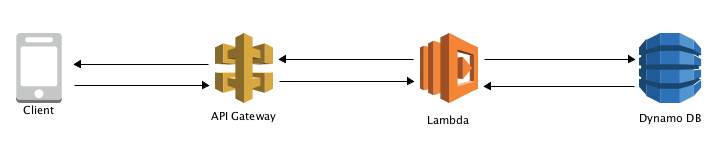
\includegraphics[width=0.5\textwidth]{high-level-overview}
\end{figure}
\section{Applicaties voor het onderzoek}
 In het onderzoek worden verschillende kleine prototypes gebruikt voor het testen van de verschillende oplossingen. Voor de client wordt steeds dezelfde applicatie gebruikt mits enkele kleine aanpassingen. Serverside wordt er gebruik gemaakt van verschillende Amazon Web Services.
\section{Client side}
De client applicatie bestaat uit een Angular applicatie, gegenereerd door Angular CLI, die verschillende synchronisatieproblemen moet voorstellen. De client vervult de rol als view voor de data die serverside wordt verwerkt. Het is niet de intentie van dit onderzoek om een volledig werkende applicatie te bouwen. Het doel van de client applicatie is om enerzijds de caching voor te stellen en anderzijds om het belang van het SSOT-principe en de store aan te tonen. Alhoewel de applicatie enkel dient als voorbeeld voor de synchronisatie, wordt er gebruik gemaakt van de design principes \autocite{brechtbilliet-scalable}\autocite{minko-gechev-scalable}. Hierbij wordt er gebruik gemaakt van een model dat verantwoordelijk is voor het uitvoeren van de requests naar de server, het opslaan en ophalen van de data naar en uit de ngrx store. Ook caching komt kort aan bod met localForage en webworkers.
\begin{figure}[h]
\caption{Flow van een client applicatie die gebruik maakt van scalable angular design patterns en AWS}
\centering
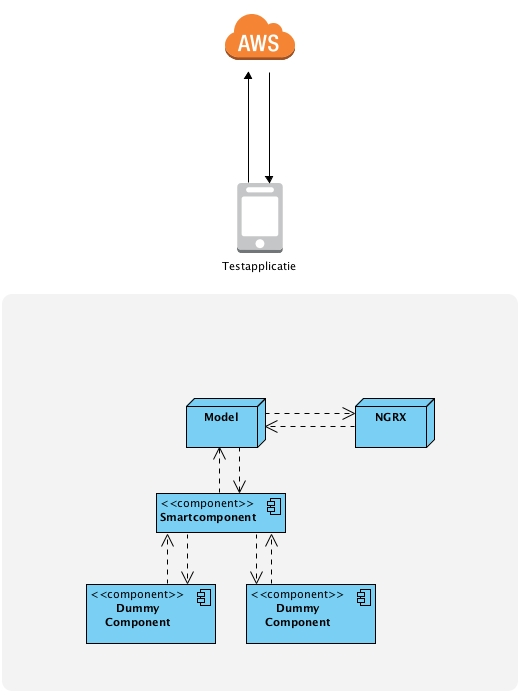
\includegraphics[width=0.5\textwidth]{testapp}
\end{figure}
\section{Server side}
Server side wordt er gebruikt gemaakt van AWS Lambda voor het verwerken van de data, SQS voor de synchronisatie en DynamoDB voor de data persistentie. Het grootste deel van de synchronisatie vindt plaatst server side dus vormt dit het omvangrijkste gedeelte van het onderzoek. Volgende afbeelding is een voorbeeld van een serverless \autocite{scalable-theorie} architectuur met de services van Amazon Web Services. Een belangrijke opmerking is dat de testomgeving geen gebruik maakt van de API-Gateway terwijl de API-Gateway service vaak\autocite{scalable-theorie}  wel wordt gebruikt bij serverless architectuur. 
\begin{figure}[h]
\caption{Voorbeeld van een serverless architectuur opgezet met verschillende Amazon Web Services}
\centering
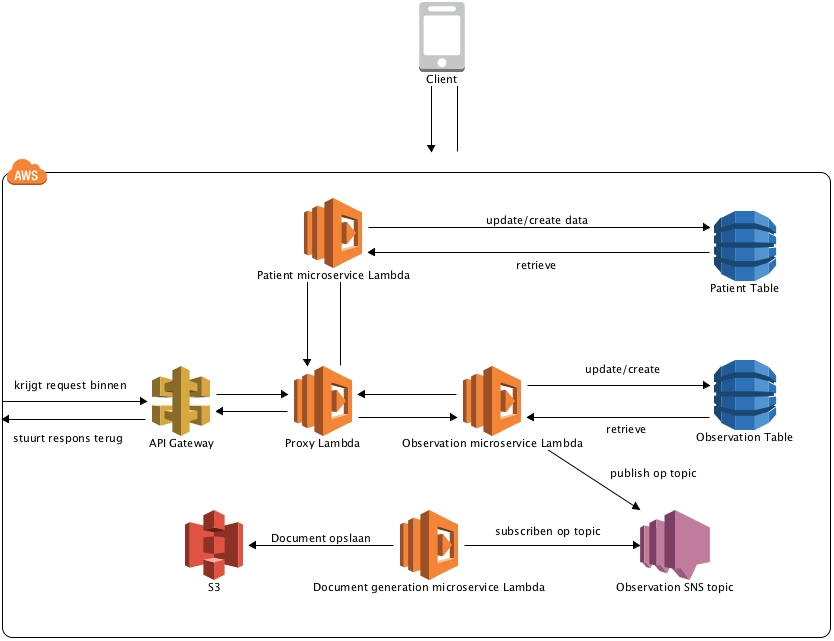
\includegraphics[width=1\textwidth]{serverless-example}
\end{figure}
